\documentclass[border=10pt,tikz]{standalone}
\usepackage{tikz}
\usetikzlibrary{positioning,arrows.meta}
\begin{document}
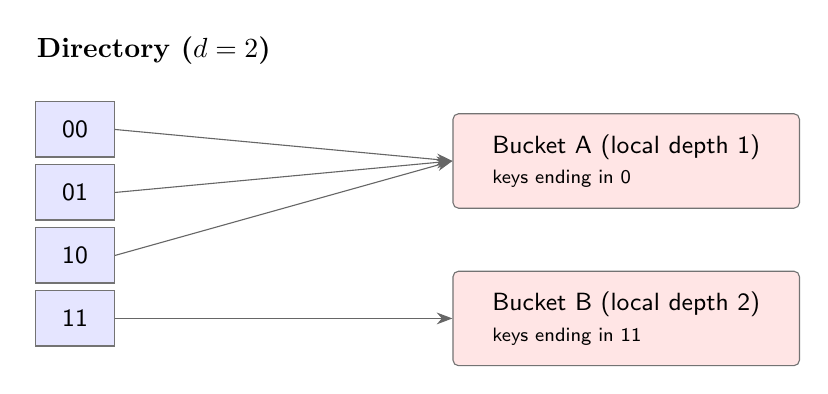
\begin{tikzpicture}[
  font=\sffamily\small,
  cell/.style={rectangle, draw=black!55, line width=0.4pt, minimum height=7mm, minimum width=10mm,
               inner sep=2pt, fill=blue!10, align=center},
  bucket/.style={rectangle, rounded corners=2pt, draw=black!55, line width=0.4pt,
                 minimum height=12mm, minimum width=44mm, inner sep=4pt, fill=red!10, align=left},
  arr/.style={-{Stealth[length=2mm]}, draw=black!60}
]
\node[draw=none, fill=none, font=\bfseries] at (-3, 3) {Directory ($d=2$)};
\node[cell] (d00) at (-4, 2) {00};
\node[cell] (d01) at (-4, 1.2) {01};
\node[cell] (d10) at (-4, 0.4) {10};
\node[cell] (d11) at (-4,-0.4) {11};

\node[bucket] (a) at (3, 1.6) {Bucket A (local depth 1) \\ \scriptsize keys ending in 0};
\node[bucket] (b) at (3,-0.4) {Bucket B (local depth 2) \\ \scriptsize keys ending in 11};

\draw[arr] (d00.east) -- (a.west);
\draw[arr] (d01.east) -- (a.west);
\draw[arr] (d10.east) -- (a.west);
\draw[arr] (d11.east) -- (b.west);
\end{tikzpicture}
\end{document}
